\documentclass{standalone}
\usepackage{tikz}
\begin{document}


\tikzset{every picture/.style={line width=0.75pt}} %set default line width to 0.75pt

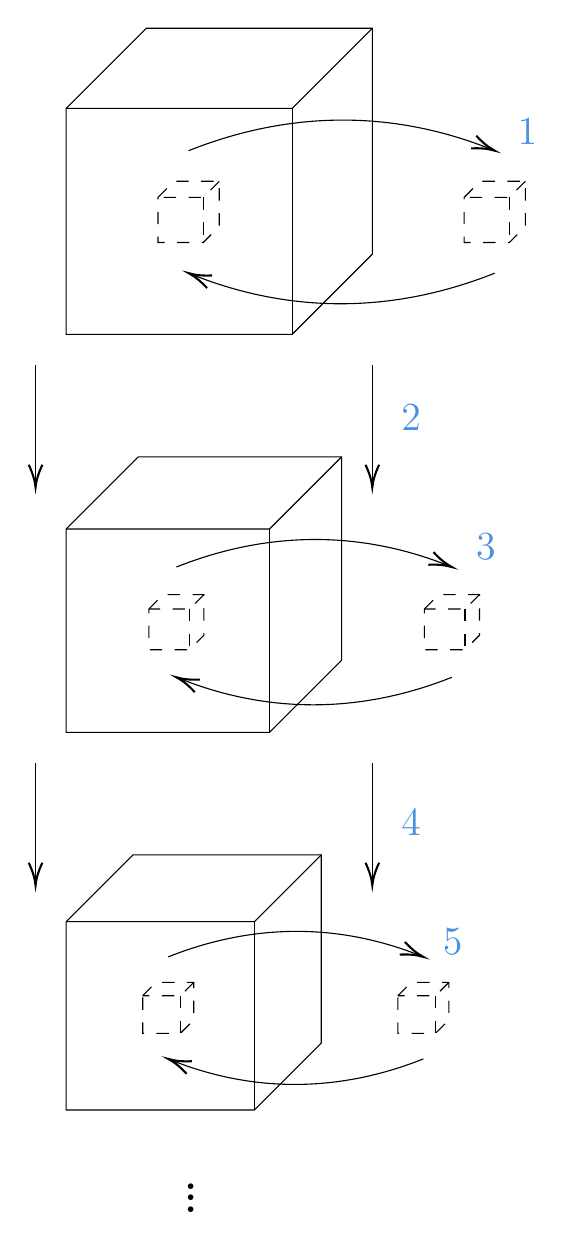
\begin{tikzpicture}[x=0.75pt,y=0.75pt,yscale=-1,xscale=1]
%uncomment if require: \path (0,651); %set diagram left start at 0, and has height of 651

%Shape: Cube [id:dp1951310418880159]
\draw   (104.75,58.63) -- (143.38,20) -- (252.25,20) -- (252.25,128.87) -- (213.62,167.5) -- (104.75,167.5) -- cycle ; \draw   (252.25,20) -- (213.62,58.63) -- (104.75,58.63) ; \draw   (213.62,58.63) -- (213.62,167.5) ;
%Shape: Cube [id:dp19330348659740637]
\draw  [dash pattern={on 4.5pt off 4.5pt}] (149,101.48) -- (156.73,93.75) -- (178.5,93.75) -- (178.5,115.52) -- (170.77,123.25) -- (149,123.25) -- cycle ; \draw  [dash pattern={on 4.5pt off 4.5pt}] (178.5,93.75) -- (170.77,101.48) -- (149,101.48) ; \draw  [dash pattern={on 4.5pt off 4.5pt}] (170.77,101.48) -- (170.77,123.25) ;
%Shape: Cube [id:dp311147726692391]
\draw  [dash pattern={on 4.5pt off 4.5pt}] (296.5,101.48) -- (304.23,93.75) -- (326,93.75) -- (326,115.52) -- (318.27,123.25) -- (296.5,123.25) -- cycle ; \draw  [dash pattern={on 4.5pt off 4.5pt}] (326,93.75) -- (318.27,101.48) -- (296.5,101.48) ; \draw  [dash pattern={on 4.5pt off 4.5pt}] (318.27,101.48) -- (318.27,123.25) ;
%Curve Lines [id:da48107672016489067]
\draw    (163.75,79) .. controls (211.94,59.81) and (261.57,59.07) .. (309.79,78.41) ;
\draw [shift={(311.25,79)}, rotate = 202.28] [color={rgb, 255:red, 0; green, 0; blue, 0 }  ][line width=0.75]    (10.93,-3.29) .. controls (6.95,-1.4) and (3.31,-0.3) .. (0,0) .. controls (3.31,0.3) and (6.95,1.4) .. (10.93,3.29)   ;
%Curve Lines [id:da9729094270445935]
\draw    (311.25,138) .. controls (263.06,157.19) and (213.43,157.93) .. (165.21,138.59) ;
\draw [shift={(163.75,138)}, rotate = 22.28] [color={rgb, 255:red, 0; green, 0; blue, 0 }  ][line width=0.75]    (10.93,-3.29) .. controls (6.95,-1.4) and (3.31,-0.3) .. (0,0) .. controls (3.31,0.3) and (6.95,1.4) .. (10.93,3.29)   ;

%Straight Lines [id:da3002419667708034]
\draw    (90,182.25) -- (90,239.25) ;
\draw [shift={(90,241.25)}, rotate = 270] [color={rgb, 255:red, 0; green, 0; blue, 0 }  ][line width=0.75]    (10.93,-3.29) .. controls (6.95,-1.4) and (3.31,-0.3) .. (0,0) .. controls (3.31,0.3) and (6.95,1.4) .. (10.93,3.29)   ;
%Straight Lines [id:da8867207825500953]
\draw    (252.25,182.25) -- (252.25,239.25) ;
\draw [shift={(252.25,241.25)}, rotate = 270] [color={rgb, 255:red, 0; green, 0; blue, 0 }  ][line width=0.75]    (10.93,-3.29) .. controls (6.95,-1.4) and (3.31,-0.3) .. (0,0) .. controls (3.31,0.3) and (6.95,1.4) .. (10.93,3.29)   ;
%Shape: Cube [id:dp20197496065494192]
\draw   (104.75,261.27) -- (139.52,226.5) -- (237.5,226.5) -- (237.5,324.48) -- (202.73,359.25) -- (104.75,359.25) -- cycle ; \draw   (237.5,226.5) -- (202.73,261.27) -- (104.75,261.27) ; \draw   (202.73,261.27) -- (202.73,359.25) ;
%Shape: Cube [id:dp8440974275393098]
\draw  [dash pattern={on 4.5pt off 4.5pt}] (144.57,299.83) -- (151.53,292.88) -- (171.13,292.88) -- (171.13,312.47) -- (164.17,319.42) -- (144.57,319.42) -- cycle ; \draw  [dash pattern={on 4.5pt off 4.5pt}] (171.13,292.88) -- (164.17,299.83) -- (144.57,299.83) ; \draw  [dash pattern={on 4.5pt off 4.5pt}] (164.17,299.83) -- (164.17,319.42) ;
%Shape: Cube [id:dp3436449451165642]
\draw  [dash pattern={on 4.5pt off 4.5pt}] (277.33,299.83) -- (284.28,292.88) -- (303.88,292.88) -- (303.88,312.47) -- (296.92,319.42) -- (277.33,319.42) -- cycle ; \draw  [dash pattern={on 4.5pt off 4.5pt}] (303.88,292.88) -- (296.92,299.83) -- (277.33,299.83) ; \draw  [dash pattern={on 4.5pt off 4.5pt}] (296.92,299.83) -- (296.92,319.42) ;
%Curve Lines [id:da5343285832320552]
\draw    (157.85,279.6) .. controls (201.22,262.33) and (245.89,261.66) .. (289.29,279.07) ;
\draw [shift={(290.6,279.6)}, rotate = 202.28] [color={rgb, 255:red, 0; green, 0; blue, 0 }  ][line width=0.75]    (10.93,-3.29) .. controls (6.95,-1.4) and (3.31,-0.3) .. (0,0) .. controls (3.31,0.3) and (6.95,1.4) .. (10.93,3.29)   ;
%Curve Lines [id:da7948824261800018]
\draw    (290.6,332.7) .. controls (247.23,349.97) and (202.56,350.64) .. (159.16,333.23) ;
\draw [shift={(157.85,332.7)}, rotate = 22.28] [color={rgb, 255:red, 0; green, 0; blue, 0 }  ][line width=0.75]    (10.93,-3.29) .. controls (6.95,-1.4) and (3.31,-0.3) .. (0,0) .. controls (3.31,0.3) and (6.95,1.4) .. (10.93,3.29)   ;

%Shape: Cube [id:dp3420743092076637]
\draw   (104.75,450.44) -- (136.94,418.25) -- (227.67,418.25) -- (227.67,508.97) -- (195.47,541.17) -- (104.75,541.17) -- cycle ; \draw   (227.67,418.25) -- (195.47,450.44) -- (104.75,450.44) ; \draw   (195.47,450.44) -- (195.47,541.17) ;
%Shape: Cube [id:dp5955054847063221]
\draw  [dash pattern={on 4.5pt off 4.5pt}] (141.63,486.15) -- (148.06,479.71) -- (166.21,479.71) -- (166.21,497.85) -- (159.77,504.29) -- (141.63,504.29) -- cycle ; \draw  [dash pattern={on 4.5pt off 4.5pt}] (166.21,479.71) -- (159.77,486.15) -- (141.63,486.15) ; \draw  [dash pattern={on 4.5pt off 4.5pt}] (159.77,486.15) -- (159.77,504.29) ;
%Shape: Cube [id:dp3568136192505327]
\draw  [dash pattern={on 4.5pt off 4.5pt}] (264.54,486.15) -- (270.98,479.71) -- (289.13,479.71) -- (289.13,497.85) -- (282.69,504.29) -- (264.54,504.29) -- cycle ; \draw  [dash pattern={on 4.5pt off 4.5pt}] (289.13,479.71) -- (282.69,486.15) -- (264.54,486.15) ; \draw  [dash pattern={on 4.5pt off 4.5pt}] (282.69,486.15) -- (282.69,504.29) ;
%Curve Lines [id:da5062438560171076]
\draw    (153.92,467.42) .. controls (193.87,451.51) and (235.02,450.81) .. (275.01,466.68) ;
\draw [shift={(276.83,467.42)}, rotate = 202.28] [color={rgb, 255:red, 0; green, 0; blue, 0 }  ][line width=0.75]    (10.93,-3.29) .. controls (6.95,-1.4) and (3.31,-0.3) .. (0,0) .. controls (3.31,0.3) and (6.95,1.4) .. (10.93,3.29)   ;
%Curve Lines [id:da23450826424555604]
\draw    (276.83,516.58) .. controls (236.88,532.49) and (195.73,533.19) .. (155.74,517.32) ;
\draw [shift={(153.92,516.58)}, rotate = 22.28] [color={rgb, 255:red, 0; green, 0; blue, 0 }  ][line width=0.75]    (10.93,-3.29) .. controls (6.95,-1.4) and (3.31,-0.3) .. (0,0) .. controls (3.31,0.3) and (6.95,1.4) .. (10.93,3.29)   ;

%Straight Lines [id:da6740933591988216]
\draw    (90,374) -- (90,431) ;
\draw [shift={(90,433)}, rotate = 270] [color={rgb, 255:red, 0; green, 0; blue, 0 }  ][line width=0.75]    (10.93,-3.29) .. controls (6.95,-1.4) and (3.31,-0.3) .. (0,0) .. controls (3.31,0.3) and (6.95,1.4) .. (10.93,3.29)   ;
%Straight Lines [id:da04414759232871934]
\draw    (252.25,374) -- (252.25,431) ;
\draw [shift={(252.25,433)}, rotate = 270] [color={rgb, 255:red, 0; green, 0; blue, 0 }  ][line width=0.75]    (10.93,-3.29) .. controls (6.95,-1.4) and (3.31,-0.3) .. (0,0) .. controls (3.31,0.3) and (6.95,1.4) .. (10.93,3.29)   ;

% Text Node
\draw (159.59,567.69) node [anchor=north west][inner sep=0.75pt] {\Huge $\vdots $};
% Text Node
\draw (321,62.4) node [anchor=north west][inner sep=0.75pt]  [font=\Large,color={rgb, 255:red, 74; green, 144; blue, 226 }  ,opacity=1 ]  {$1$};
% Text Node
\draw (265,200.4) node [anchor=north west][inner sep=0.75pt]  [font=\Large,color={rgb, 255:red, 74; green, 144; blue, 226 }  ,opacity=1 ]  {$2$};
% Text Node
\draw (301,262.4) node [anchor=north west][inner sep=0.75pt]  [font=\Large,color={rgb, 255:red, 74; green, 144; blue, 226 }  ,opacity=1 ]  {$3$};
% Text Node
\draw (265,395.4) node [anchor=north west][inner sep=0.75pt]  [font=\Large,color={rgb, 255:red, 74; green, 144; blue, 226 }  ,opacity=1 ]  {$4$};
% Text Node
\draw (285,452.4) node [anchor=north west][inner sep=0.75pt]  [font=\Large,color={rgb, 255:red, 74; green, 144; blue, 226 }  ,opacity=1 ]  {$5$};


\end{tikzpicture}
\end{document}